\documentclass[12pt]{article}

\usepackage{amsmath}
\usepackage{graphicx}
\usepackage{amssymb}
\usepackage{mathrsfs}
\usepackage{geometry}
\usepackage{color}
\usepackage{verbatimbox}
\geometry{margin=2cm}

\usepackage{hyperref}
\hypersetup{
    colorlinks=true,
    linkcolor=blue,
    filecolor=magenta,      
    urlcolor=cyan,
}

\usepackage{url}
\usepackage{tcolorbox}
\usepackage{multirow}
\usepackage{float}

\usepackage{setspace}
\onehalfspacing

\newcommand\tab[1][1cm]{\hspace*{#1}}


\title{Modifying All-Silicon Tracker Prototype in EICroot}
\author{Reynier Cruz Torres}

\begin{document}

\maketitle

\tableofcontents

% ========================================================================================
\newpage
\section{Accessing EICroot image}

EICroot and necessary dependencies are already installed in a virtual machine.
Install VMware.
Double click on the file \verb|vm-eic.vmx|.
When the image loads, it will ask for a username (eic) and password (eiceic).
This virtual machine was created with the Beast detector geometry. Thus, two files (\verb|vst.C| and \verb|fbst.C|) need to be updated
so that the code generates the All-Silicon tracker geometry instead. The original codes I got from Yue Shi Lai are appended at the end of this document.

% ========================================================================================
\section{Modifying the geometry}

The All-Si tracker geometry is defined in: \verb|Home/eicroot/geometry/|.

% ========================================
\subsection{Beampipe}

The beam-pipe geometry is defined in:

\begin{tcolorbox}
\begin{verbatim}
Home/eicroot/geometry/BEAMPIPE/beampipe.C
\end{verbatim}  
\end{tcolorbox}

The central part of the beampipe is made of Beryllium and is 800 $\mu$m thick.
It is 36 mm in diameter, and extends from -400 to 400 mm:

\begin{tcolorbox}
\begin{verbnobox}[\scriptsize]
BeamPipeElement *ip = new BeamPipeElement("beryllium", 0.800);
ip->AddSection(-400.0, 36.00);
ip->AddSection( 400.0, 36.00);
\end{verbnobox}  
\end{tcolorbox}

Outside of this range, the beampipe becomes Aluminum and extends from where the Beryllium section ends and up until $\pm$4.5 m.
it increases in diameter from 36 mm to 40 mm:

\begin{tcolorbox}
\begin{verbnobox}[\scriptsize]
BeamPipeElement *p1 = new BeamPipeElement("aluminum", 1.000);
p1->AddSection( 400.0,  36.00);
p1->AddSection(1000.0,  40.00);
p1->AddSection(4500.0,  40.00);
\end{verbnobox}  
\end{tcolorbox}

This is how the geometry is defined. Then it is assembled as follows:

\begin{tcolorbox}
\begin{verbnobox}[\scriptsize]
BeamPipeGeoParData *bpipe = new BeamPipeGeoParData();
bpipe->AddElement  (p1, BeamPipeElement::Swap);
bpipe->AddIpElement(ip);
bpipe->AddElement  (p1);
\end{verbnobox}  
\end{tcolorbox}

Fig.~\ref{fig:beampipe} shows a diagram for the beampipe.

\begin{figure}[H]
\centering
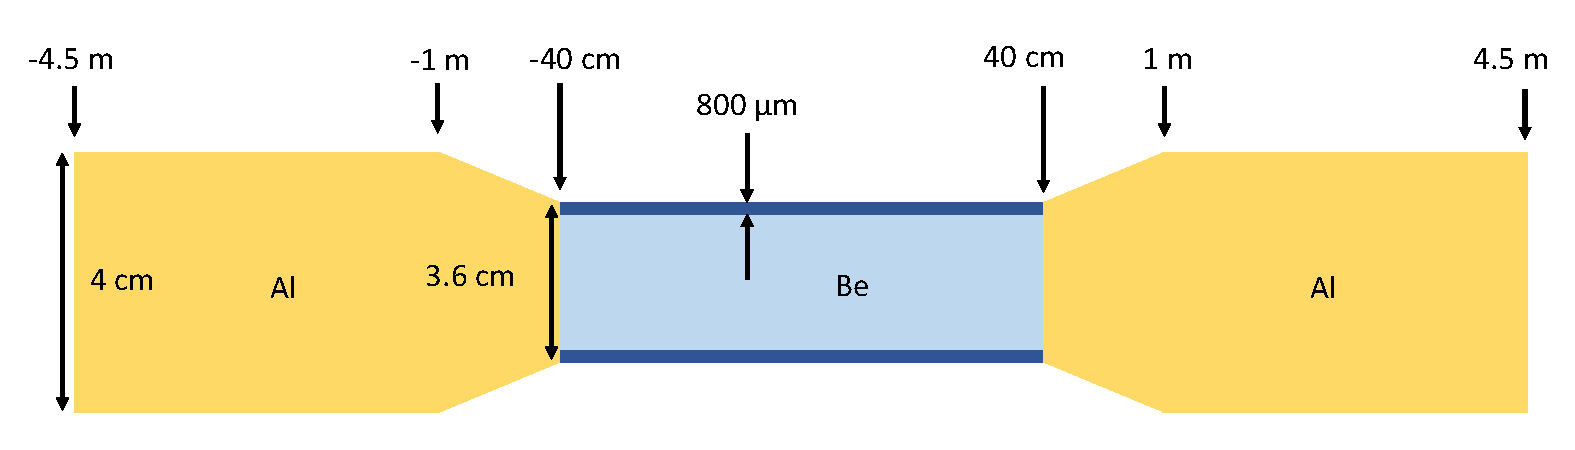
\includegraphics[width=0.6\textwidth]{figures/beampipe.pdf}
\caption{Beampipe schematic (not in scale).}
\label{fig:beampipe}
\end{figure}

% ========================================
\subsection{Barrel}

The barrel details are in:

\begin{tcolorbox}
\begin{verbatim}
Home/eicroot/geometry/MAPS/vst.C
\end{verbatim}  
\end{tcolorbox}

The first step is to define the common cell that will be used to build up the barrel:

\begin{tcolorbox}
\begin{verbnobox}[\scriptsize]
MapsMimosaAssembly *ibcell = (MapsMimosaAssembly*)ConfigureAliceCell();
\end{verbnobox}  
\end{tcolorbox}

Then, six layers are assembled, as illustrated below. The variables passed in \verb|AddBarrelLayer| below correspond to:
cell assembly type,
number of staves in this layer,
number of chips in a stave,
chip center installation radius,
additional stave slope around beam line direction in degrees,
layer rotation around beam axis ``as a whole'' in degrees:

\begin{tcolorbox}
\begin{verbnobox}[\scriptsize]
vst->AddBarrelLayer(ibcell,   12     ,  9     ,    23.4, 12.0, 0.0);
vst->AddBarrelLayer(ibcell, 2*12     ,  9     ,  2*23.4, 12.0, 0.0);

vst->AddBarrelLayer(ibcell, 6*12     , 14     ,  6*23.4, 14.0, 0.0);
vst->AddBarrelLayer(ibcell, 4*20     , 14     ,  4*39.3, 14.0, 0.0);

vst->AddBarrelLayer(ibcell, 4*20*10/4, 14*10/4, 10*39.3, 14.0, 0.0);
vst->AddBarrelLayer(ibcell, 4*20*11/4, 14*11/4, 11*39.3, 14.0, 0.0);
\end{verbnobox}  
\end{tcolorbox}

The information in this snippet of code is presented in Table~\ref{tab:barrel}.
An overall overview of the barrel geometry is shown in Fig.~\ref{fig:geom} a).

\begin{table}[H]
\centering
\caption{Barrel characteristics}
\label{tab:barrel}
\begin{tabular}{c|ccccc}
\hline
\multirow{2}{*}{Layer} & \# staves  & \# chips  &length along& chip center                     & stave slope \\
                                   &  in layer    & in stave  &z (cm)        & installation radius (mm) & (deg) \\
\hline \hline
1       			 & 12             & 9            & 27              & 23.4                            & 12                \\
2        			 & 24             & 9            & 27              & 46.8                            & 12                \\
3       			 & 72             & 14          & 42              & 140.4                           & 14                \\
4       			 & 80             & 14          & 42              & 157.2                           & 14                \\
5        			 & 200           & 35          & 105            & 393                             & 14                \\
6        			 & 220           & 38          & 114            & 432.3                           & 14               
\end{tabular}
\end{table}

\begin{figure}
\centering
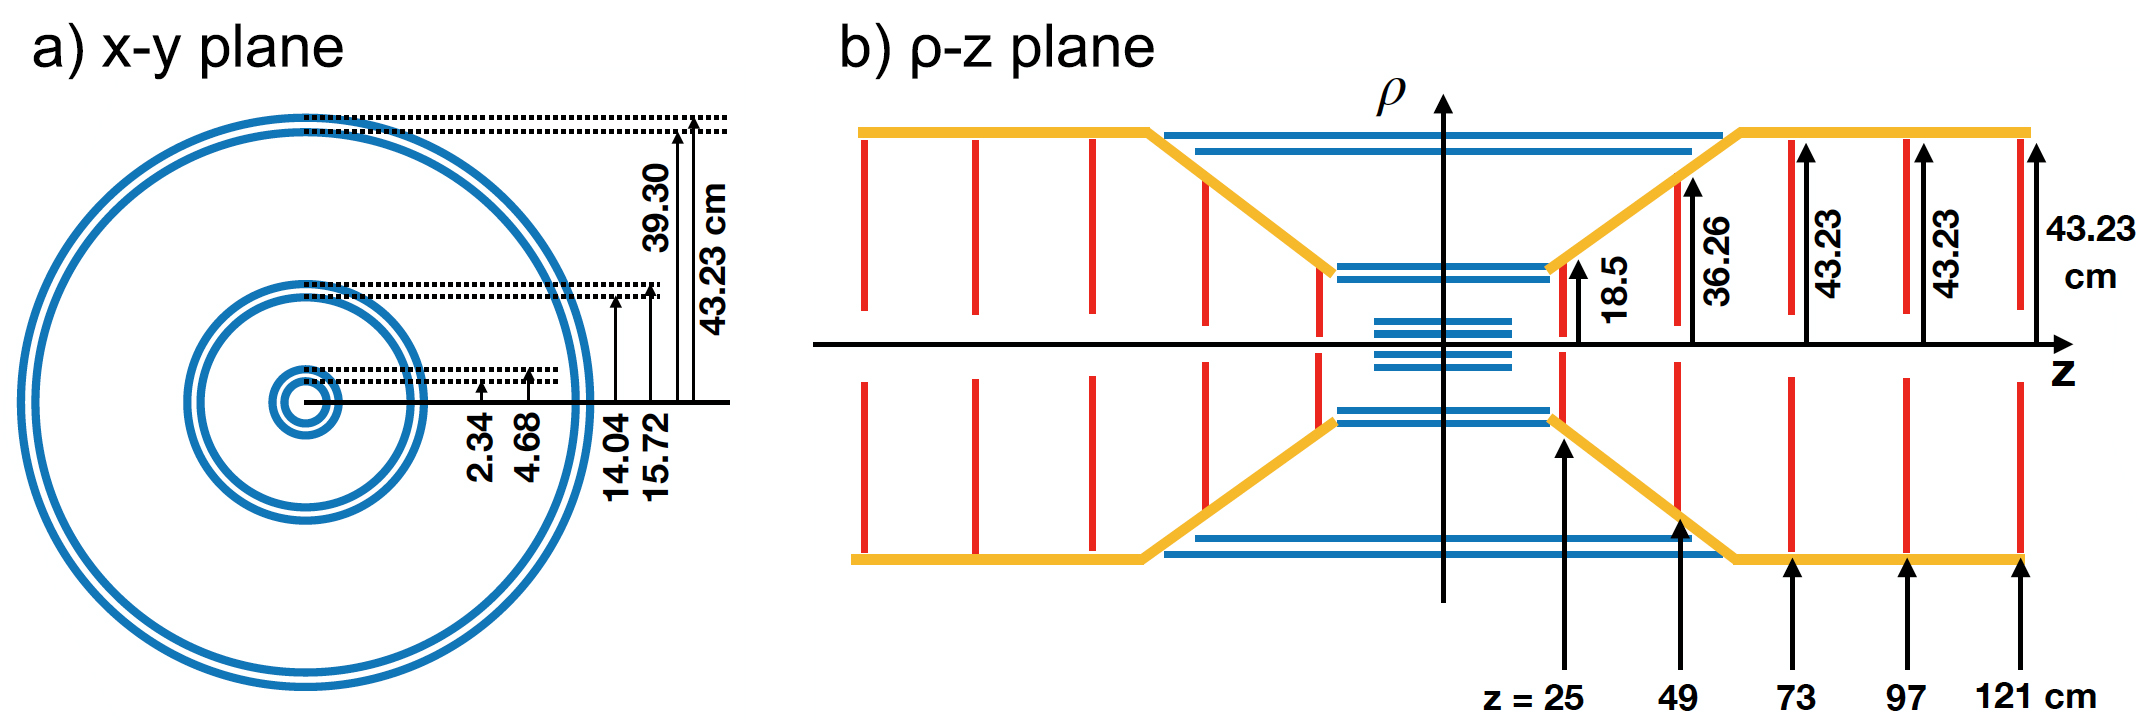
\includegraphics[width=\textwidth]{figures/geometry_details.jpg}
\caption{Schematic of the detector geometry. The barrel, disks, and support structure are drawn in blue, red, and yellow respectively.
a) barrel as seen in the $x-y$ plane. b) detector as seen in the $\rho-z$ plane.
This is a simplified diagram, as the barrel layers and disks are not smooth. The barrel is formed by staves, and the disks have jagged edges.}
\label{fig:geom}
\end{figure}

Here, a ``chip'' refers to a Mimosa chip assembly, and is the basic building block for the detector.
The chip characteristics are defined in:

\begin{tcolorbox}
\begin{verbnobox}[\scriptsize]
Home/eicroot/geometry/MAPS/maps-lib.C
\end{verbnobox}  
\end{tcolorbox}

The chips are defined with a width of 15 mm and a length (in z) of 30 mm. Consequently, the length of the barrel layers in z is given by
the number of chips per stave and corresponds to \verb|(# chips)|$\times$\verb|(chip length)|.

% ========================================
\subsection{Disks}

The disks are in:

\begin{tcolorbox}
\begin{verbatim}
Home/eicroot/geometry/MAPS/fbst.C
\end{verbatim}  
\end{tcolorbox}

At the top of this code we define the number of disks we will have in each z direction:

\begin{tcolorbox}
\begin{verbnobox}[\scriptsize]
#define _DISK_NUM_ (5)
\end{verbnobox}  
\end{tcolorbox}

Then, the positions in z and radii of these disks are determined as follows:

\begin{tcolorbox}
\begin{verbnobox}[\scriptsize]
Double_t Z[_DISK_NUM_];
Double_t R[_DISK_NUM_];
for (size)t i = 0; i  < _DISK_NUM_; i++) {
      Z[i] = 250 + i * (1210.0 - 250.0) / (_DISK_NUM_ - 1);
      R[i] = 45.0 * (i % 2);
}
\end{verbnobox}  
\end{tcolorbox}

This corresponds to the values shown in Table~\ref{tab:disks}
and in Fig.~\ref{fig:geom} b).

\begin{table}[H]
\centering
\caption{Disk characteristics (in the forward direction). To get backward disks multiply the z-position column by -1.}
\label{tab:disks}
\begin{tabular}{c|cc}
\hline
Disk number & z position {[}cm{]} & outer radius {[}cm{]} \\
\hline \hline
1           & 25                  & 18.5                  \\
2           & 49                  & 36.26                 \\
3           & 73                  & 43.23                 \\
4           & 97                  & 43.23                 \\
5           & 121                 & 43.23                
\end{tabular}
\end{table}

The disks are added the following way:

\begin{tcolorbox}
\begin{verbnobox}[\scriptsize]
for(unsigned dc=0; dc<_DISK_NUM_; dc++) {
    FstDisc *disc = new FstDisc(ibcell, 18.0, TMath::Min(432.3, 185.0 * Z[dc] / Z[0]), 12.8);
    fbst->AddDisc(disc, (fb ? -1.0 : 1.0)*Z[dc], R[dc]);
}
\end{verbnobox}  
\end{tcolorbox}    

% ========================================
\subsection{Support structure}

\color{red}
Note: EICroot uses millimeters as the standard length unit. All the lengths shown up to this point corresponded to mm.
However, the support structure is defined directly using Geant classes, which use cm as the standard length unit.
Thus, the lengths in this section are given in cm.
\color{black}

The support structure is also defined in:

\begin{tcolorbox}
\begin{verbatim}
Home/eicroot/geometry/MAPS/fbst.C
\end{verbatim}  
\end{tcolorbox}

The parameters that go into \verb|DefineSection| are: a numeric tag or label, z position, inner radius, and outer radius.
The support structure is defined with three sections. 

\begin{tcolorbox}
\begin{verbnobox}[\scriptsize]
TGeoPcon *support = new TGeoPcon("AluStrips_support", 0.0, 360,0, 3);

support->DefineSection(0, (fb ? 1.0 : -1.0) * 20 , 18.5 * 20.0 / 25.0 , 18.5 *  20.0 / 25.0 + 0.5);
support->DefineSection(1, (fb ? 1.0 : -1.0) * 43.23 * 0.1 * Z[0] / 18.5, 43.23, 43.23 + 0.5);
support->DefineSection(2, (fb ? 1.0 : -1.0) * 121, 18.5 * 121.0 / 25.0, 18.5 * 121.0 / 25.0 + 0.5);

TGeoVolume *support_volume = new TGeoVolume("AluStrips_support_volume", support, fbst->GetMedium("aluminum"));

fbst->GetTopVolume()->AddNode(support_volume, 0, new TGeoCombiTrans(0.0, 0.0, 0.0, 0));
\end{verbnobox}  
\end{tcolorbox}

% ========================================================================================
\section{Compiling the geometry into a TGeo file}

First of all, run the macros mentioned above. Go to the corresponding directories and run:

\begin{itemize}
\item \verb|root -l beampipe.C|
\item \verb|root -l vst.C|
\item \verb|root -l fbst.C|
\end{itemize}
This will create root files that contain these pieces of the geometry to be stored in the combined TGeo file.
Next, edit the function \verb|void EicDetector::FinishRun()| in code:

\begin{tcolorbox}
\begin{verbatim}
Home/eicroot/eic/base/EicDetector.cxx
\end{verbatim}  
\end{tcolorbox}

to include the following three lines (add as the first three lines of that function):

\begin{tcolorbox}
\begin{verbnobox}[\scriptsize]
TFile *outfile = TFile::Open("genfitGeom.root","RECREATE");
gGeoManager->Write();
outfile->Close();
\end{verbnobox}  
\end{tcolorbox}

Afterwards, you have to recompile by \verb|make -C build| or \verb|cd Home/eicroot/eic/build; make|.

Run the following root macro to compile the geometry:

\begin{tcolorbox}
\begin{verbnobox}[\scriptsize]
{
        // Load basic libraries;
        gROOT->Macro("$VMCWORKDIR/gconfig/rootlogon.C");

        // Create simulation run manager; use GEANT3 for tracking excercises here;
        EicRunSim *fRun = new EicRunSim("TGeant3");
        fRun->SetOutputFile("simulation-uds.root");

        // Vertex tracker;
        fRun->AddModule(new EicMaps   ("VST", "/home/eic/eicroot/geometry/MAPS/vst-v01.0-fs.root", qVST)); 
        fRun->AddModule(new EicMaps   ("FST", "/home/eic/eicroot/geometry/MAPS/fst-v01.0-ns.root", qFST)); 
        fRun->AddModule(new EicMaps   ("BST", "/home/eic/eicroot/geometry/MAPS/bst-v01.0-ns.root", qBST)); 

        // Beam pipe; details of IR not known yet -> just a cylinder with thin walls;
        fRun->AddModule(new EicDummyDetector("BEAMPIPE", "BEAMPIPE/beampipe.root"));

        // Initialize and run the simulation; exit at the end;
        fRun->Run(-1);
} 
\end{verbnobox}  
\end{tcolorbox}

% ========================================================================================
\section{Visualizing the geometry}

\begin{tcolorbox}
\begin{verbnobox}[\scriptsize]
{
        // Load basic libraries;
        gROOT->Macro("$VMCWORKDIR/gconfig/rootlogon.C");

        // Create simulation run manager; use GEANT3 for tracking excercises here;
        EicRunSim *fRun = new EicRunSim("TGeant3");
        fRun->SetOutputFile("simulation-uds.root");

        // Vertex tracker;
        fRun->AddModule(new EicMaps   ("VST", "/home/eic/eicroot/geometry/MAPS/vst-v02.0-fs.root", qVST));
        fRun->AddModule(new EicMaps   ("FST", "/home/eic/eicroot/geometry/MAPS/fst-v02.0-ns.root", qFST));
        fRun->AddModule(new EicMaps   ("BST", "/home/eic/eicroot/geometry/MAPS/bst-v02.0-ns.root", qBST));

        // Beam pipe; details of IR not known yet -> just a cylinder with thin walls;
        fRun->AddModule(new EicDummyDetector("BEAMPIPE" , "/home/eic/eicroot/geometry/BEAMPIPE/beampipe.root"));

        // Initialize and run the simulation; exit at the end;
        fRun->Run(1);
}
\end{verbnobox}  
\end{tcolorbox}

\begin{tcolorbox}
\begin{verbnobox}[\scriptsize]
{
  gROOT->Macro("$VMCWORKDIR/gconfig/rootlogon.C"); // Load basic libraries;

  // Create visualization manager; 
  EicEventManager *fMan = new EicEventManager();
  fMan->SetInputFile("simulation-uds.root");

  fMan->Init(); // Initialize and run visualization manager; tune vis.properties a bit;

  fMan->Run();
}
\end{verbnobox}  
\end{tcolorbox}

\begin{figure}
\centering
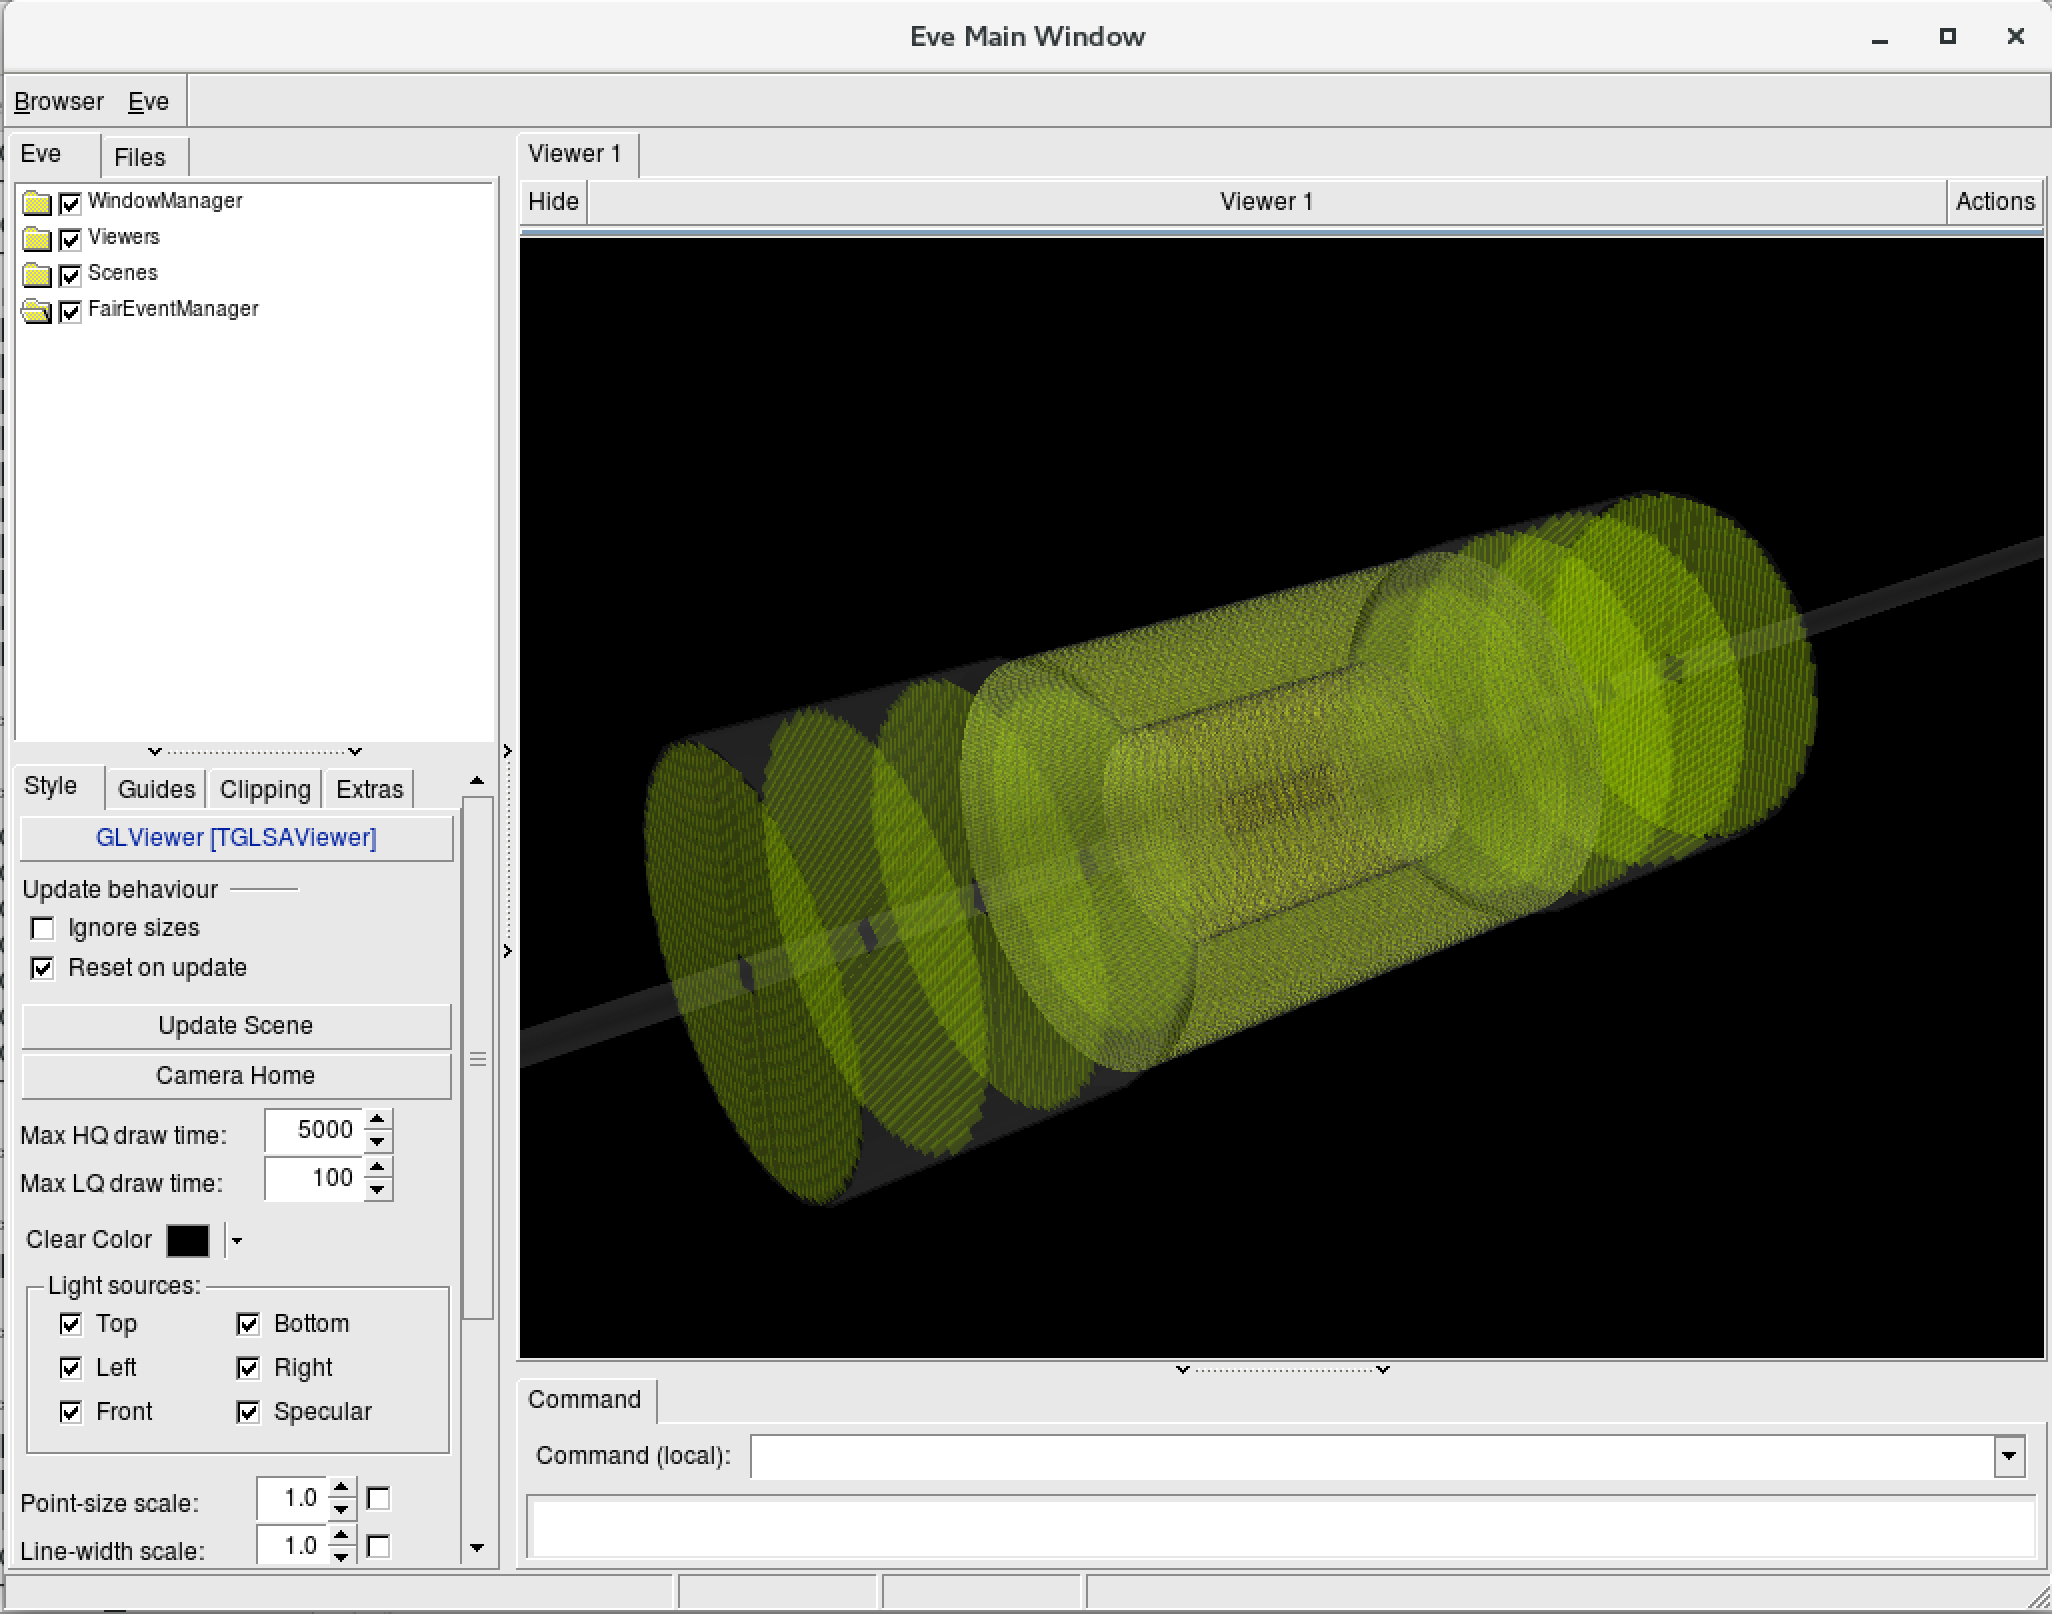
\includegraphics[width=0.5\textwidth]{figures/viewer.png}
\caption{Event-display GUI.}
\label{fig:visual}
\end{figure}

% ========================================================================================
\section{Detector updates (week of July 13-17, 2020)}

\subsection{Beampipe updates}

\begin{tcolorbox}
\begin{verbnobox}[\scriptsize]
BeamPipeElement *ip = new BeamPipeElement("beryllium", 0.762);
ip->AddSection(-798.0, 62.00);
ip->AddSection( 798.0, 62.00);

BeamPipeElement *pf = new BeamPipeElement("aluminum", 1.000);
pf->AddSection(  798.0, 62.00);
pf->AddSection( 4500.0, 62.00);

bpipe->AddElement  (pf,BeamPipeElement::Swap);
bpipe->AddIpElement(ip);
bpipe->AddElement  (pf);
\end{verbnobox}  
\end{tcolorbox}

\subsection{Barrel updates}

Below are two possible upgrades for the barrel. Tho innermost layers are identical in these two upgrades,
and differ from the original configuration in that their radii and number of staves have been increased to accommodate the
beampipe.

Upgrade 1:

This version has the two middle and two outer layers configured such that the triangular
staves are back-to-back. See Fig.~\ref{fig:barrel_upgrades} (center).
\begin{tcolorbox}
\begin{verbnobox}[\scriptsize]
vst->AddBarrelLayer(ibcell,  17,      10,  32.000,  12.0, 0.0        );
vst->AddBarrelLayer(ibcell,2*13,      10,  40.000,  12.0, 0.0        );

vst->AddBarrelLayer(ibcell,  82,      20, 224.700,   0.5, 0.0        );
vst->AddBarrelLayer(ibcell,  82,      20, 228.980, 179.5, 180/82     );

vst->AddBarrelLayer(ibcell, 151, 14*10/4, 413.985,   0.5,         0.0);
vst->AddBarrelLayer(ibcell, 151, 14*10/4, 419.095, 179.5, 180/151+0.2);
\end{verbnobox}  
\end{tcolorbox}

Upgrade 2:

This version has the two middle and two outer layers configured such that the silicon part of each stave
faces one another. See Fig.~\ref{fig:barrel_upgrades} (right). This makes the detector more hermetic.
\begin{tcolorbox}
\begin{verbnobox}[\scriptsize]
vst->AddBarrelLayer(ibcell,  17,      10,  32.000,  12.0, 0.0        );
vst->AddBarrelLayer(ibcell,2*13,      10,  40.000,  12.0, 0.0        );

vst->AddBarrelLayer(ibcell,  82,      20, 224.700,   0.5, 0.0        );
vst->AddBarrelLayer(ibcell,  82,      20, 224.200, 179.5, 180/82     );

vst->AddBarrelLayer(ibcell, 151, 14*10/4, 419.510,   0.5,         0.0);
vst->AddBarrelLayer(ibcell, 151, 14*10/4, 419.095, 179.5, 180/151+0.2);
\end{verbnobox}  
\end{tcolorbox}

Additionally, with respect to the original barrel, some of the length of the staves in z has been changed
to reflect the changes in the rest of the geometry.

\begin{figure}[H]
\centering
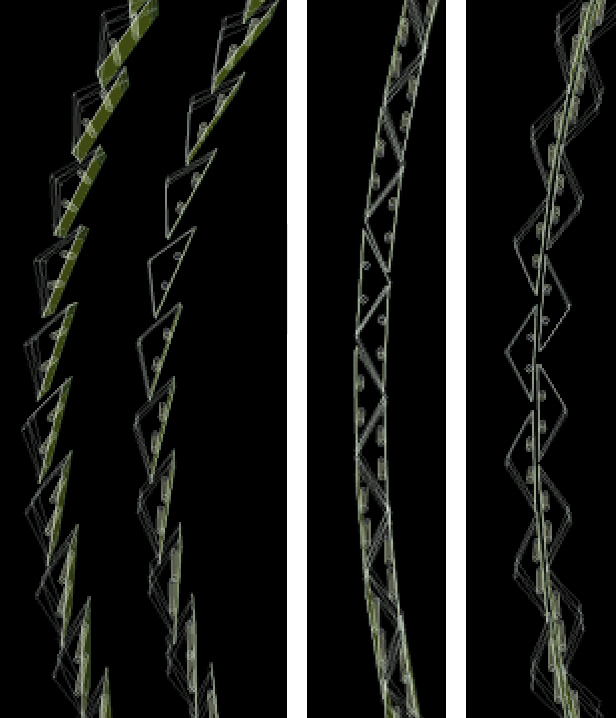
\includegraphics[width=0.3\textwidth]{figures/barrel_upgrades.jpg}
\caption{Different configurations for the barrel layers: (left) original, (center) upgrade 1, and (right) upgrade 2.}
\label{fig:barrel_upgrades}
\end{figure}

\subsection{Disk updates (Under Construction)}

In order to avoid these gaps, a ``hack'' was implemented. The mimosa chips were extended in width.








































% ========================================================================================
\pagebreak
\appendix
\section{Appendices}
\subsection{Original vst.C macro from Yue Shi Lai}

\begin{tcolorbox}
\begin{verbnobox}[\tiny]
#define _VERSION_     1
#define _SUBVERSION_  0

//#define _TEST_VERSION_ // Do not want to always overwrite "official" files; place "test" tag into the file name;

// All construction elements are smeared (so chip assembly is uniform in both beam line and asimuthal direction); 
//#define _NO_STRUCTURE_GEOMETRY_
// No tricky elements like inclined roof beams; still water pipes, etc are 
// created (so chip assembly is uniform in beam line direction only);
//#define _BEAM_LINE_UNIFORM_GEOMETRY_

#define _USE_TRIANGULAR_ASSEMBLIES_ // In case of VST no need to fall back to tricky TGeoCompositeShape cell assemblies;

//#define _WITH_MOUNTING_RINGS_ // Comment out if no mounting rings wanted;
//#define _WITH_ENFORCEMENT_BRACKETS_ // Comment out if no stave enforcement brackets wanted;
//#define _WITH_EXTERNAL_PIPES_ // Comment out if no external water pipe pieces wanted;

#include <geometry/MAPS/maps-lib.C>

vst()
{
  // Load basic libraries;
  gROOT->Macro("$VMCWORKDIR/gconfig/rootlogon.C");

  // Prefer to think in [mm] and convert to [cm] when calling ROOT shape 
  // definition routines only;

  VstGeoParData *vst = new VstGeoParData(_VERSION_, _SUBVERSION_);

  // Parse #define statements and make certain configuration calls accordingly;
  // NB: cast to the base MAPS geo class since void* interface used; FIXME!; 
  DefinitionParser((MapsGeoParData*)vst);

  // For now assume ALICE Inner Barrel design only (but with more than 9 chips); no problem to introduce similar design with a bit different
  // parameter set later; construction a-la ALICE Outer Barrel looks like an overkill to the moment;

  // No offset per default;
  //vst->SetTopVolumeTransformation(new TGeoTranslation(0.0, 0.0, 0.0));

  // NB: all these numbers are sort of arbitrary; allow to get better visual representation, but do not reflect any reality of the final design;

  // Mounting ring construction; arbitrary numbers, same for all layers;
  if (vst->WithMountingRings()) {
    vst->mMountingRingBeamLineThickness =    5.00;
    vst->mMountingRingRadialThickness   =    5.00;
    vst->mMountingRingRadialOffset      =    3.00;
  } //if
  // Simplify the design -> just a triangular piece with a reasonable volume; 
  if (vst->WithEnforcementBrackets())
    vst->mEnforcementBracketThickness   =    1.00;
  // This is something for display purposes mostly;
  if (vst->WithExternalPipes())
    vst->mWaterPipeExtensionLength      =    4.00;

  MapsMimosaAssembly *ibcell = (MapsMimosaAssembly*)ConfigureAliceCell();

  // If (much) longer staves needed, create an enforced configuration;
  //MapsMimosaAssembly *obcell = new MapsMimosaAssembly(ibcell);
  //obcell->mEnforcementBeamDiameter     =    1.00; ... and so on ...

  // Now when basic building blocks are created, compose barrel layers;
  // a dirty part, but perhaps the easiest (and most readable) to do; parameters are:
  //  - cell assembly type;
  //  - number of stoves in this layer;
  //  - number of chips in a stove;
  //  - chip center installation radius;
  //  - additional stove slope around beam line direction; [degree];
  //  - layer rotation around beam axis "as a whole"; [degree];
  //
  vst->AddBarrelLayer(ibcell,   12,  9,   23.4, 12.0, 0.0);
  vst->AddBarrelLayer(ibcell, 2*12,  9, 2*23.4, 12.0, 0.0);

  vst->AddBarrelLayer(ibcell, 6*12, 14, 6*23.4, 14.0, 0.0);
  vst->AddBarrelLayer(ibcell, 4*20, 14, 4*39.3, 14.0, 0.0);

  vst->AddBarrelLayer(ibcell, 4*20*10/4, 14*10/4, 10*39.3, 14.0, 0.0);
  vst->AddBarrelLayer(ibcell, 4*20*11/4, 14*11/4, 11*39.3, 14.0, 0.0);

  vst->AttachSourceFile("vst.C");
  vst->AttachSourceFile("maps-lib.C");
  vst->AttachSourceFile("../../eic/detectors/maps/VstGeoParData.cxx");

  // Specify color preferences; NB: void* interface, sorry;
  SetMapsColors((EicGeoParData*)vst);

  //
  // Fine, at this point structure is completely defined -> code it in ROOT;
  //

  vst->ConstructGeometry();

  // Yes, always exit;
  exit(0);
}
\end{verbnobox}  
\end{tcolorbox}

% ========================================================================================
\pagebreak
\subsection{Original fbst.C file from Yue Shi Lai}

\begin{tcolorbox}
\begin{verbnobox}[\tiny]
#define _VERSION_     1
#define _SUBVERSION_  0

//#define _TEST_VERSION_ // Do not want to always overwrite "official" files; place "test" tag into the file name;

// All construction elements are smeared (so chip assembly is uniform in both beam line and asimuthal direction);
#define _NO_STRUCTURE_GEOMETRY_ 

// No tricky elements like inclined roof beams; still water pipes, etc are created (so chip assembly is uniform in beam line direction only);
#define _BEAM_LINE_UNIFORM_GEOMETRY_ 

// FIXME: does not work; in case of FST/BST will have to fall back to tricky TGeoCompositeShape cell assemblies; also half of the cells should be
// Z-rotated to bring chips close to the beam pipe;
#define _USE_TRIANGULAR_ASSEMBLIES_

//#define _WITH_MOUNTING_RINGS_ // Comment out if no mounting rings wanted;
//#define _WITH_ENFORCEMENT_BRACKETS_ // Comment out if no stave enforcement brackets wanted;
//#define _WITH_EXTERNAL_PIPES_ // Comment out if no external water pipe pieces wanted;

#include <geometry/MAPS/maps-lib.C>

#define _DISK_NUM_  (5)

fbst()
{
  // Load basic libraries;
  gROOT->Macro("$VMCWORKDIR/gconfig/rootlogon.C");

  Double_t Z[_DISK_NUM_];
  Double_t R[_DISK_NUM_];
  for (size_t i = 0; i < _DISK_NUM_; i++) {
     Z[i] = 250 + i * (1210.0 - 250.0) / (_DISK_NUM_ - 1);
     R[i] = 45.0 * (i % 2);
  }

  for(unsigned fb=0; fb<2; fb++) {
    FstGeoParData *fbst = new FstGeoParData(fb ? "BST" : "FST", _VERSION_, _SUBVERSION_);

    // Parse #define statements and make certain configuration calls accordingly;
    // NB: cast to the base MAPS geo class since void* interface used; FIXME!; 
    DefinitionParser((MapsGeoParData*)fbst);

    // Prefer to think in [mm] and convert to [cm] when calling ROOT shape definition routines only;

    // Mounting ring construction; arbitrary numbers, same for all layers;
    if (fbst->WithMountingRings()) {
      fbst->mMountingRingBeamLineThickness =    3.00;
      fbst->mMountingRingRadialThickness   =    5.00;
    } //if
   
    if (fbst->WithEnforcementBrackets()) // Simplify the design -> just a triangular piece with a reasonable volume; 
      fbst->mEnforcementBracketThickness   =    1.00;
    // This is something for display purposes mostly;
    if (fbst->WithExternalPipes())
      fbst->mWaterPipeExtensionLength      =    4.00;

    //  For now assume ALICE Inner Barrel design, composed in stoves with varying number of Mimosa chips;

    MapsMimosaAssembly *ibcell = (MapsMimosaAssembly*)ConfigureAliceCell();

    // For now consider a single disc design (all the same); add stoves by hand;
    // Parameters: cell assembly pointer, min available radius, max available radius, default neigboring stave overlap in "X" direction;

    // Declare discs; just put them by hand at hardcoded locations along the beam line;
    for(unsigned dc=0; dc<_DISK_NUM_; dc++) {
      FstDisc *disc = new FstDisc(ibcell, 18.0, TMath::Min(432.3, 185.0 * Z[dc] / Z[0]), 12.8);

      fbst->AddDisc(disc, (fb ? -1.0 : 1.0)*Z[dc], R[dc]);
    }
#if 0
    if (!fb) {
      FstDisc *hdisc = new FstDisc(ibcell, 18.0, 400.0, 12.8);

      fbst->AddDisc(hdisc, 1500.);
    } //if
#endif

    fbst->AttachSourceFile("fbst.C");
    fbst->AttachSourceFile("maps-lib.C");
    fbst->AttachSourceFile("../../eic/detectors/maps/FstGeoParData.cxx");

#if 1
    TGeoPcon *support = new TGeoPcon("AluStrips_support", 0.0, 360.0, 3);

    support->DefineSection(0, (fb ? 1.0 : -1.0) * 20, 18.5 * 20.0 / 25.0, 18.5 * 20.0 / 25.0 + 0.5);
    support->DefineSection(1, (fb ? 1.0 : -1.0) * 43.23 * 0.1 * Z[0] / 18.5, 43.23, 43.23 + 0.5);
    support->DefineSection(2, (fb ? 1.0 : -1.0) * 121, 43.23, 43.23 + 0.5);

    TGeoVolume *support_volume = new TGeoVolume("AluStrips_support_volume", support, fbst->GetMedium("aluminum"));

    fbst->GetTopVolume()->AddNode(support_volume, 0, new TGeoCombiTrans(0.0, 0.0, 0.0, 0));
#endif

    // Specify color preferences; NB: void* interface, sorry;
    SetMapsColors((EicGeoParData*)fbst);

    // Geometry is defined -> build it in ROOT;
    fbst->ConstructGeometry();
  } //for fb
  
  exit(0);
}
\end{verbnobox}  
\end{tcolorbox}

% ========================================================================================
\pagebreak
\subsection{Help menu from event display GUI}

\begin{figure}[H]
\centering
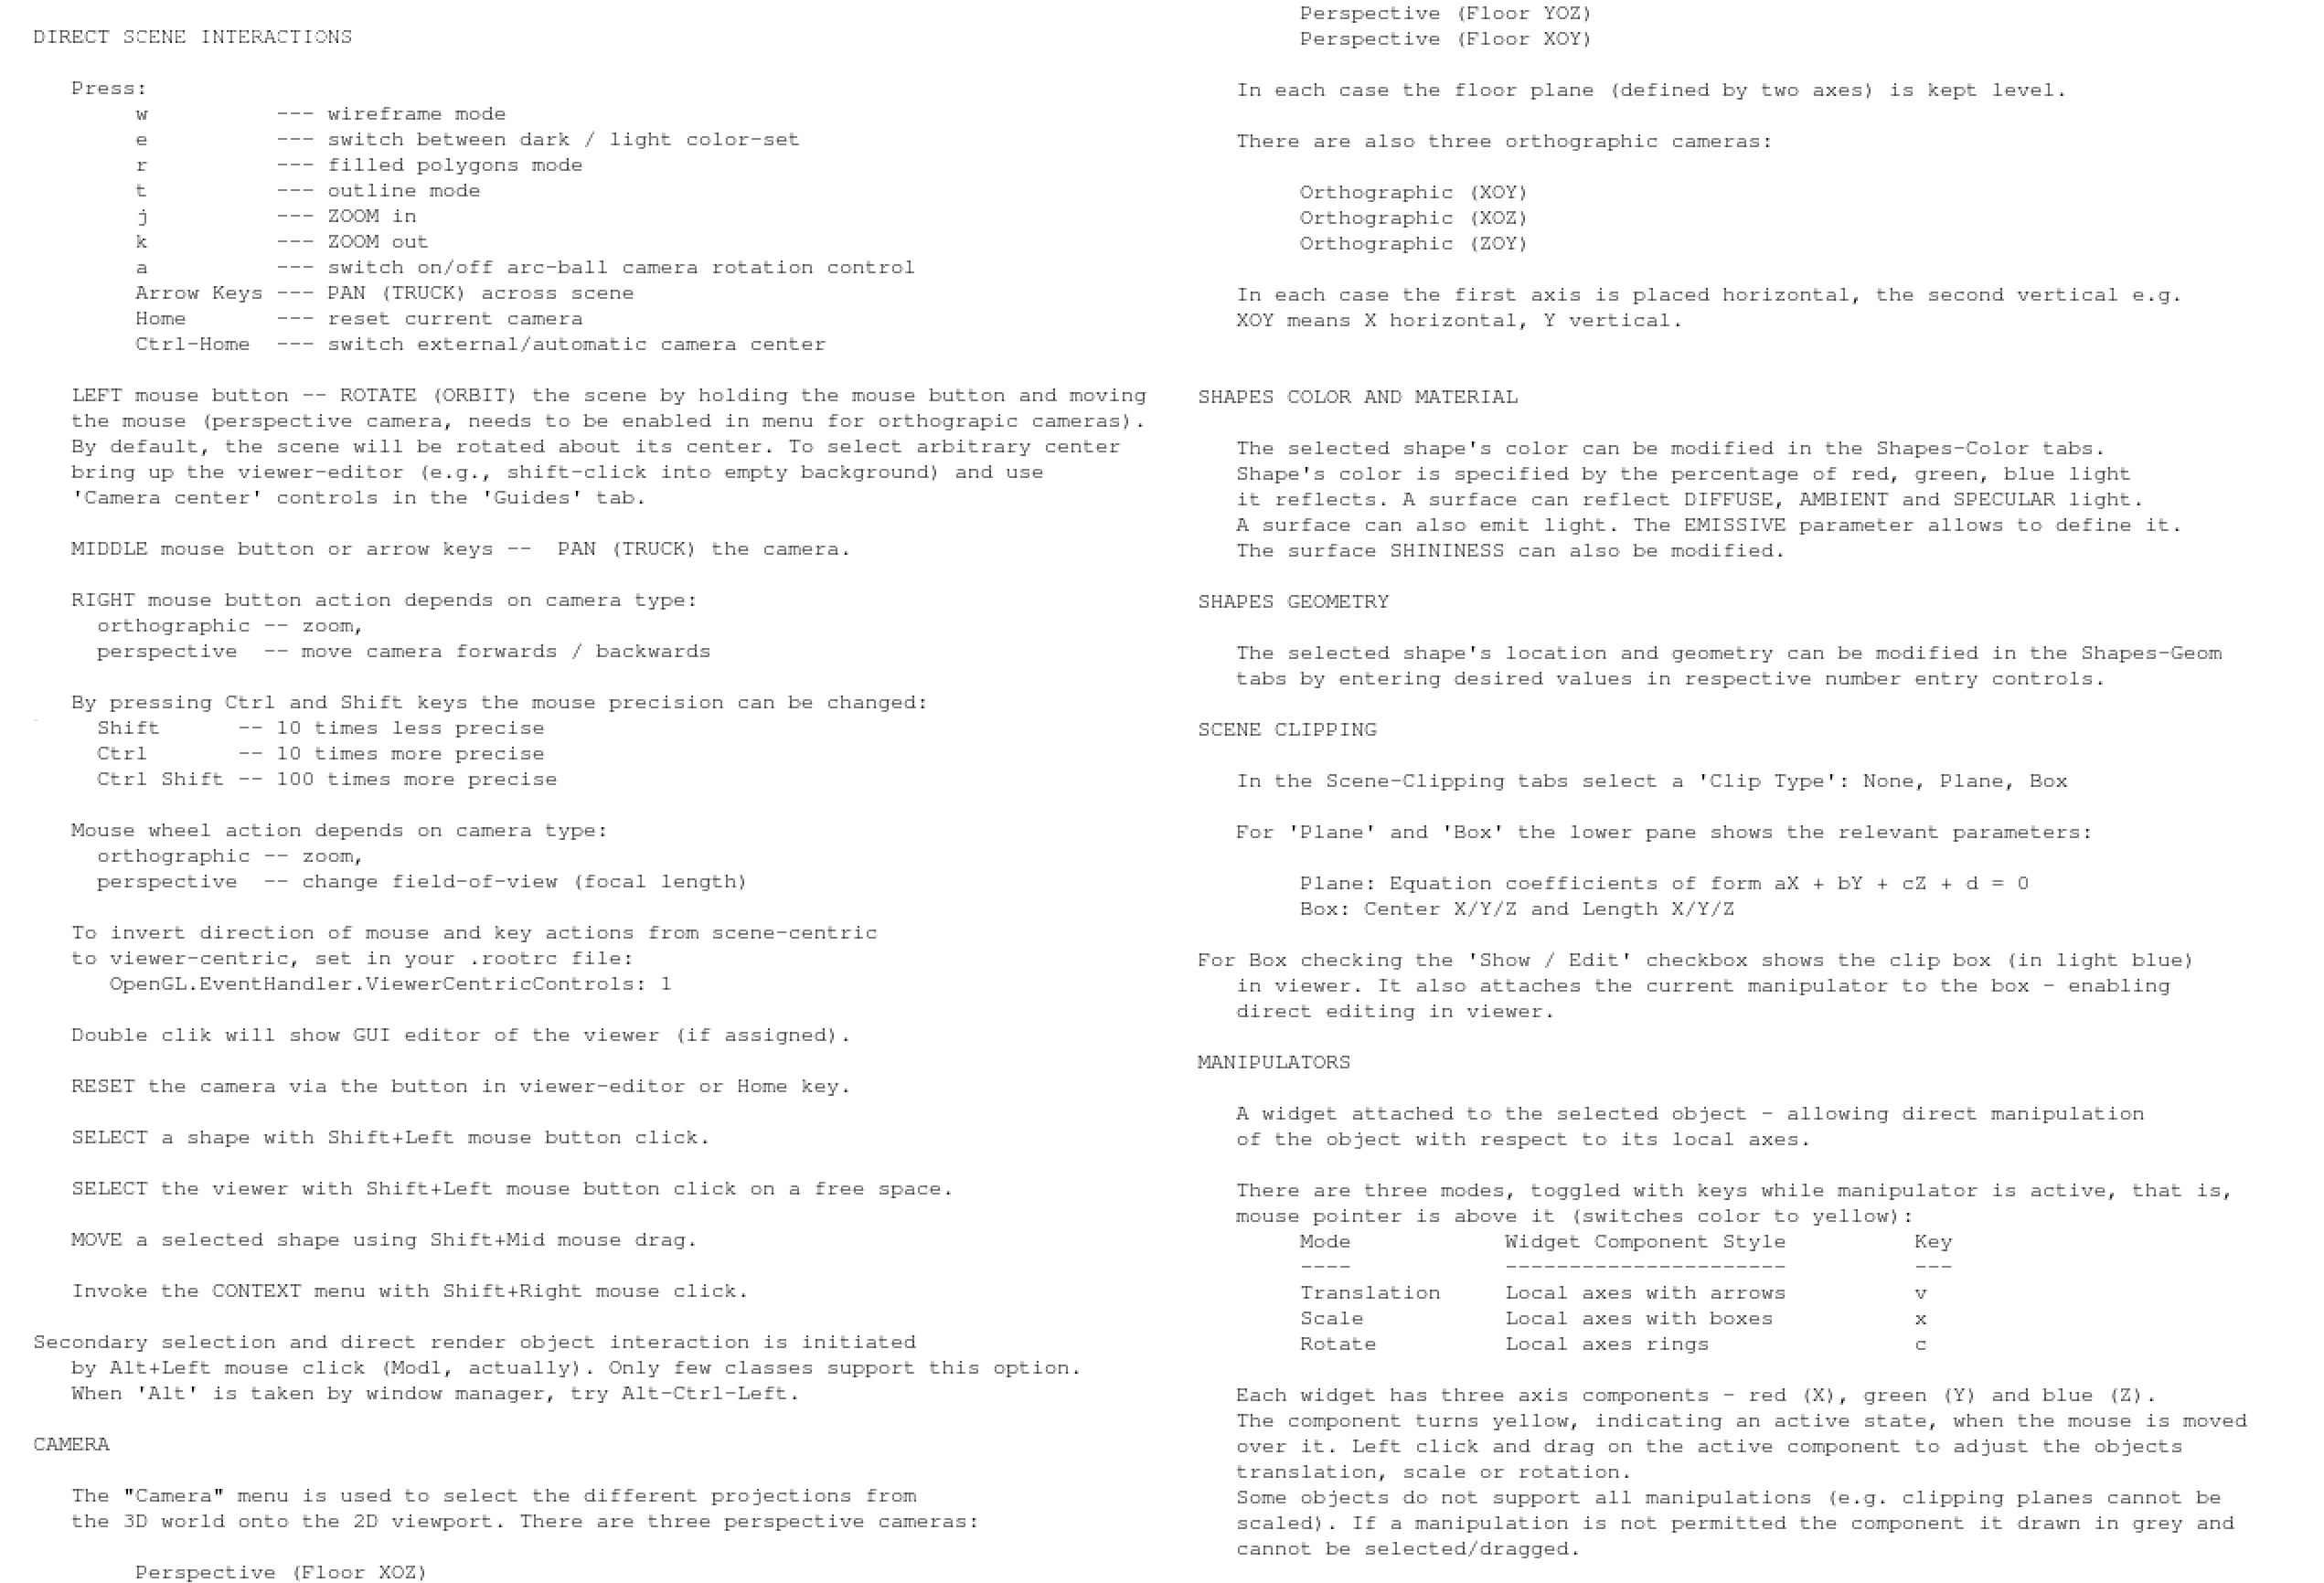
\includegraphics[width=\textwidth]{figures/viewer_help.jpg}
\caption{Event-display GUI help menu.}
\label{fig:visual_help}
\end{figure}

%\bibliography{bib_file}
%\bibliographystyle{ieeetr}

\end{document}





